\chapter*{2023年\textsf{\textsc{Hdu}}「普通物理2」期中试题}

\vspace{-12.0pt}\setcounter{page}{1}
\begin{center}
  \begin{minipage}{.66\textwidth}
    \centering
    \begin{tasks}
      [ label-width = 5\ccwd, item-indent = 2cm,
        after-item-skip = 0pt ](2)
      \task[\textbf{课程信息}：] 理学院/A0715022
      \task[\textbf{授课教师}：] 陈许敏
      \task[\textbf{解析提供}：] \textsf{Skyrmion}
      \task[{\makebox[5em][s]{\textbf{\textsf\TeX~排版}：}}] \textsf{Skyrmion}
    \end{tasks}
  \end{minipage}
  \begin{minipage}{.15\textwidth}
    \centering
    \begin{tikzpicture}
      \node [ inner sep = 0 ] (wechat) {
        \fancyqr
          [ size = 4em, image padding = 1,
            image = \raisebox{4em/33}{\textcolor{DarkGreen}{\faIcon{weixin}}},
            r color = DarkGreen, version = 4
          ]{http://weixin.qq.com/r/sRJiemTEGjllrSAZ90ej}
        };
      \node [ inner sep = .5ex, align = center, right, font = \scriptsize ]
        at (wechat.east) {未\\央\\学\\社};
    \end{tikzpicture}
  \end{minipage}
  \begin{minipage}{.15\textwidth}
    \centering
    \begin{tikzpicture}
      \node [ inner sep = 0 ] (qq) {
        \fancyqr
          [ size = 4em, image x padding = 2, image y padding = 1,
            image = \raisebox{4em/33}{\textcolor{MidnightBlue}{\faIcon{qq}}},
            l color = MidnightBlue, version = 4
          ]{https://qm.qq.com/q/PH7CsQWvm2}
        };
      \node [ inner sep = .5ex, align = center, left, font = \scriptsize ]
        at (qq.west) {物\\理\\营};
    \end{tikzpicture}
  \end{minipage}
\end{center}

\section{Part A（每空3分，共30分）}

\begin{problem}
  一个小球与轻弹簧组成的系统做简谐运动，若 $t = 0$ 时，小球位于平衡点处，
  且向正 $x$ 轴方向运动，则小球简谐运动的初相位是 \result{$-\pi/2$}.
\end{problem}
\begin{solution}
  $t = 0$ 时 $x = 0,~ v > 0$，画出相图比对得 $\phi_0 = -\pi/2$.
\end{solution}

\begin{problem}
  一个质点同时参与两个方向、同频率的简谐振动：
  $x_1 = 0.4\cos(\pi t + \pi/6),~ x_2 = 0.3\cos(\pi t + \phi_{20})$.
  当 $\phi_{20} = $ \result{$\pi/6$}（$-\pi < \phi_{20} < \pi$）时，
  该质点合振动的振幅最大，合振幅为 \result{$0.7$}.
\end{problem}
\begin{solution}
  两振动初相相同时合振幅最大，所以 $\phi_{20} = \pi/6$. 合振幅为
  $A = \sqrt{A_1^2 + A_2^2 + 2A_1A_2\cos\Delta\phi_0} = 0.7$.
\end{solution}

\begin{problem}
  自然光和线偏振光组成的混合光束强度之比为 $1:3$，通过一偏振片时，
  随着偏振片以光的传播方向为轴的转动，透射光的最强和最弱的光强之比为 \result{$7:1$}.
\end{problem}
\begin{solution}
  自然光透过偏振片后光强为原来的 $50\%$，线偏振光透过偏振片后光强最大为$100\%$，
  最弱为$0\%$. 则由此得透射光的最强和最弱的光强之比为
  $(1 \times 50\% + 3 \times 100\%):(1 \times 50\% + 3 \times 0\%) = 1:7$.
\end{solution}

\begin{problem}
  杨氏双缝干涉实验中，两缝相距 $\qty2\mm$，屏离缝的距离为 $\qty1\m$，入射光的波长为
  $\qty{500}\nm$，则相邻明纹中心的间距是 \result{$\qty{250}\um$}；如果用折射率
  $n_1 = 1.58$ 的云母片遮盖一条缝，屏幕上的零级亮纹移到原来的第 $6$ 级明纹位置上，
  则云母片的厚度为 \result{$\qty{5.17}\um$}.
\end{problem}
\begin{solution}
  相邻明纹中心间距 $\Delta x = \lambda f/a = \qty{250}\um$；
  云母片遮盖后光程差的变化为 $6\lambda = e(1.58 - 1)$，
  由此可得云母片的厚度为 $\qty{5.17}\um$.
\end{solution}

\begin{problem}
  设月光的波长为 $\qty{600}\nm$，若在地球上用物镜直径为 $\qty2\m$ 的天文望远镜观察时，
  刚能分辨月球正面上的距离为 $\qty{140.5}\m$ 的两点，
  则地球到月球的距离是 \result{$\qty{3.84e5}\km$}.
\end{problem}
\begin{solution}
  由望远镜的最大分辨本领 $\Delta x = 1.22\lambda l/D$ 得
  $l = D\Delta x/1.22\lambda = \qty{3.84e5}\km$.
\end{solution}

\begin{problem}
  在一条笔直的公路上，一警车正鸣笛追赶着违法肇事车辆驾车逃逸的一摩托车驾驶员.
  摩托车的速率为 $\qty{36}{\km/\hour}$，警车的速率为 $\qty{72}{\km/\hour}$.
  假设空气中没有风，空气中的声音速度为 $u = \qty{330}{\m/\s}$，
  警笛声音的频率为 $\qty{500}\Hz$.
  摩托车驾驶员听到的警笛声的频率是 \result{$\qty{516.13}\Hz$}，
  摩托车驾驶员观测到的警笛声的波长是 \result{$\qty{0.62}\m$}.
\end{problem}
\begin{solution}
  观察者 (Observer) 远离，所以 $v_o < 0$；发射源 (Source) 接近，所以 $v_s < 0$.
  由多普勒效应公式得观察者所听频率为
  \[
    f = \frac{u \pm v_o}{u \mp v_s}\nu_0
      = \frac{330 - 10}{330 - 20} \times \qty{500}\Hz \approx \qty{516.13}\Hz
  \]
  摩托车驾驶员观测到的警笛的波长 $\lambda_o = (u - v_o)/f = \qty{0.62}\m$.
\end{solution}

\begin{problem}
  波长 $\lambda = \qty{600}\nm$ 的单色光照射宽 $a = \qty{0.5}\mm$ 的单缝上，
  在单缝后放一个焦距 $f = \qty{0.5}\m$ 的凸透镜，屏幕放置在焦距处.
  中央亮条纹的宽度为 \result{$\qty{1.2}\mm$}.
\end{problem}
\begin{solution}
  中央亮条纹的宽度 $\Delta x_0 = 2\lambda f/a = \qty{1.2}\mm$.
\end{solution}

\section{Part B（每题10分，共40分）}

\begin{textfig}
  \begin{problem}
    一个振动质点的振动曲线如图所示，试求
    \begin{enumerate}
      \item 简谐振动的位移方程.
      \item 质点从振动开始位置到 $P$ 点所需的时间.
    \end{enumerate}
  \end{problem}
  \textfigsplit\centering
  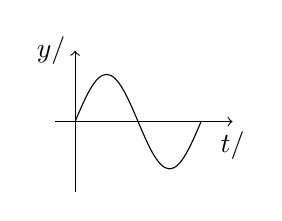
\begin{tikzpicture}
    \draw [ -> ] (-.25,0) -- (2,0) node [ below ] {$t/\unit\s$};
    \draw [ -> ] (0,-.9) -- (0,.9) node [ left ] {$y/\unit\m$};
    \draw (0,0) sin (.4,.6) cos (.8,0) sin (1.2,-.6) cos (1.6,0);
  \end{tikzpicture}
\end{textfig}

\begin{problem}
  一平面单色光在空气中以 $i_1 = \qty{30}\degree$ 照射到厚度均匀的薄油膜上.
  油膜覆盖在玻璃板上，所用单色光的波长可以连续变化
\end{problem}
\begin{solution}\leavevmode
\begin{enumerate}
  \item $t = 0$ 时 $y = 0,~ v > 0,~ \phi_0 = -\pi/2$.
  所以位移方程为 $y = 0.04\cos\ab(5\pi t - \pi/2)$.
  \item $P$ 点相位 $\phi_P = 11\pi/6$，
  质点运动到 $P$ 点用时 $t = \phi_P/\omega = \qty{0.37}\s$.
\end{enumerate}
\end{solution}

\section{Part C（每题15分，共30分）}

% \begin{problem}[薄膜干涉]
%     一平面単色光在空气中以$i_1=30^\circ$照射到厚度均匀的薄油膜上.油膜覆盖在玻璃板上，所用单色光的波长可以连续变化，观察到$500\mathrm{nm}$ 与$600\mathrm{nm}$这两个波长的光在反射中干涉叠加，亮度显著增强.油的折射率为$1.30$，玻璃的折射率为$1.50$.试求油膜的最小厚度.
% \end{problem}
% \begin{solution}
% \begin{itemize}
%     \item 由折射定律$n_1=\sin i_1=n_2\sin i_2$得$\cos i_2=\cos\arcsin\frac{n_1\sin i_1}{n_2}=0.92$.
%     \item 设两波长的光在第$k$级叠加增强，光程差满足$2n_2h\cos i_2=k\lambda_1=(k+1)\lambda_2$，则$k$满足的最小正整数为$k=5$.
%     \item 将$k=5$代入得油膜的最小厚度$h_{\min}=\frac{k\lambda_1}{2n_2\cos i_2}=1.25\mu\mathrm{m}$.
% \end{itemize}
% \end{solution}

% \begin{paracol}{2}
% \begin{problem}[平面简谐波的波函数]
%     如图所示为一平面简谐波在$t=2\mathrm{s}$时刻的波形图，$u=0.6\mathrm{m/s}$，求
% \begin{enumerate}
%     \item 坐标原点$O$质点的振动方程.
%     \item 该波的波函数.
%     \item $P$点振动方程.
% \end{enumerate}
% \end{problem}
% \switchcolumn\centering
% \vfill
% \begin{tikzpicture}[decoration={markings,
%     mark=between positions 0.05 and 1 step 6mm
%     with {\draw [-,gray] (0,-0.1) -- (0,0.1);}}]
%     \draw [thick,->,postaction=decorate] (-0.2,0)--(4.2,0) node [anchor=south] {$x/\mathrm{m}$};
%     \draw [thick,->] (0,-1.2)--(0,1.5) node [anchor=south] {$y/\mathrm{m}$};
%     \node [anchor=north east] at (0,0) {$O$};
%     \draw [thick] (0,0) sin (0.6,-1) cos (1.2,0) sin (1.8,1) node [anchor=south] {$t=2\mathrm{s}$} cos (2.4,0) sin (3,-1) cos (3.6,0);
%     \draw [very thick,<-] (2.4,1.2)--(3.6,1.2) node [anchor=south,midway] {$u$};
%     \node [anchor=north] at (1.2,0) {$0.3$};
%     \draw [densely dotted,thick] (0,-1)--(1.2,-1) node [anchor=east,at start] {$0.04$};
%     \shade[ball color=H1] (1.2,0) circle (.05) node [anchor=south east] {$P$};
% \end{tikzpicture}
% \vfill
% \end{paracol}
% \begin{solution}
% \begin{enumerate}
%     \item 由图可知振幅$A=0.04\mathrm{m}$，角频率$\omega=\frac{2\pi u}{\lambda}=2\pi$，初相$\varphi=\frac\pi2$. 所以原点的振动方程为\point{2}
%     \[y_o=0.04\cos\ab(2\pi(t-2)+\frac\pi2)=0.04\cos\ab(2\pi t+\frac\pi2)\eqno\point{2}\]
%     \item $y=0.04\cos\ab[2\pi\ab(t-2+\frac{x}{0.6})+\frac\pi2]=0.04\cos\ab[2\pi\ab(t+\frac{5x}{3})+\frac\pi2]$.\point{3}
%     \item 将$x=0.3$代入波函数得$y_p=0.04\cos\ab(2\pi t-\frac\pi2)$.\point{3}
% \end{enumerate}
% \end{solution}

% \begin{problem}[光栅]
%     波长为$500\mathrm{nm}$的单色平行光垂直入射到一个透射光栅上，第三级明纹出现在$\sin\theta=0.5$处，第四级缺级. 试求
% \begin{enumerate}
%     \item 光栅常数$d$是多少？
%     \item 光栅上狭缝可能的最小宽度$a$有多大？
%     \item 在光屏上观察到最高谱线级次是多少？
%     \item 在光屏上可以看到哪些级数的谱线？
% \end{enumerate}
% \end{problem}
% \begin{solution}
% \begin{enumerate}
%     \item 由光栅方程$d\sin\theta=k\lambda$得$d=\frac{k\lambda}{\sin\theta}=3\mu\mathrm{m}$.\point{3}
%     \item 由缺级条件$k'=\frac da$得$a=\frac d4=0.75\mu\mathrm{m}$.\point{2}
%     \item 分别令$\sin\theta=\pm 1$得$k=\pm 6$. 由于现实中$\sin\theta$取不到$1$，所以可见最高级次为$5$.\point{3}
%     \item $\pm 3$级缺级，所以可见谱线级数有$0,\ \pm1,\ \pm2,\ \pm4,\ \pm5$.\point{2}
% \end{enumerate}
% \end{solution}

% \section*{第3部分（每题15分，共30分）}
% \begin{problem}[驻波]
%     平面简谐波沿$x$轴正方向传播，频率$f=100\mathrm{Hz}$，振幅$A=0.1\mathrm{m}$，波速$u=100\mathrm{m/s}$.已知在$t=0$时刻，距离坐标原点$x_1=0.5\mathrm{m}$处的质点的位移为$0.1\mathrm{m}$. 当传播到$x_2=2\mathrm{m}$处的固定端时，被全部反射，且反射点是节点. 假设入射波和反射波具有相同的振幅，圆频率和波长. 试求
% \begin{enumerate}
%     \item 入射波的波函数.
%     \item 反射波的波函数.
%     \item 合成波的波函数.
%     \item 合成波在$0\leq x\leq 2$区间内，波腹和波节点的横坐标.
% \end{enumerate}
% \end{problem}
% \begin{solution}
% \begin{enumerate}
%     \item $y_1=0.1\cos\ab[200\pi\ab(t-\frac{x-0.5}{100})]=0.1\cos\ab[200\pi\ab(t-\frac{x}{100})+\pi]$.\point{3}
%     \item $y_2=0.1\cos\ab[200\pi\ab(t-\frac{2}{100}+\frac{x-2}{100})]=0.1\cos\ab[200\pi\ab(t+\frac{x}{100})]$.\point{5}
%     \item $y=y_1+y_2=0.2\cos\ab(200\pi t+\frac\pi2)\cos\ab(2\pi x-\frac\pi2)$.\point{3}
%     \item 分别令$\cos\ab(2\pi x-\frac\pi2)=\pm1,\ 0$得此区间内波腹坐标$x=\frac14,\ \frac34,\ \frac54,\ \frac74$，波节坐标$x=0,\ \frac12,\ 1,\ \frac32,\ 2$.\point{4}
% \end{enumerate}
% \end{solution}

% \vskip-2ex
% \begin{paracol}{2}
% \begin{problem}[简谐振动]
%     一个光滑水平面上的弹簧振子，弹簧的劲度系数为$k=900.0\mathrm{N/m}$，弹簧的质量为$m_s=0.3\mathrm{kg}$. 所系物体的质量为$m=0.9\mathrm{kg}$，物块的振幅$A=0.1\mathrm{m}$. 有一质量为$M=8.0\mathrm{kg}$的小物体从高度$h=0.5\mathrm{m}$处自由下落，如图所示. 当振子在最大正位移时，小物体落在物块上，并粘在一起. 假设碰撞在极短时间内完成，也就是碰撞过程中弹簧长度不发生改变. 假定弹簧各截面的位移是线性的. 试求
% \begin{enumerate}
%     \item 碰撞前，物体经过平衡位置时，物体的速率.
%     \item 碰撞前，系统的振动周期.
%     \item 碰撞后，物体经过平衡位置时，物体的速率.
%     \item 碰撞后，系统的振动周期.
% \end{enumerate}
% \end{problem}
% \switchcolumn\centering
% \vfill
% \begin{tikzpicture}
%     \draw [->] (0,1) -- (0,0) -- (5,0) node [anchor=north] {$x$};
%     \draw (2.1,.8) -- (2.1,-.3) node [near end,anchor=north east] {$O$};
%     \draw (3,.8) -- (3,-.3) node [near end,anchor=north east] {$A$};
%     \draw [decorate,decoration={coil,segment length=3pt}] (0,.3) -- (2.7,.3) node [near start,anchor=south] {$m_2$};
%     \filldraw [fill=1号色] (2.7,0) rectangle (3.3,.6);
%     \node [anchor=west] at (3.3,.3) {$m$};
%     \shade [ball color=H1] (3.3,3) circle (.1) node [anchor=east] {$M$};
%     \length{(3.6,.6)}{(3.6,3)}{$h$}{(0,.5)}
% \end{tikzpicture}
% \vfill
% \end{paracol}
% \vspace{-.75em}
% \begin{solution}
% \begin{itemize}
%     \item 弹簧的动能$T=\frac12\int_0^l\frac{m_s}{l}\ab(\frac{vx}{l})^2\d x=\frac16m_sv^2=\frac12m_\text{eff}v^2$，由此得弹簧的有效质量$m_\text{eff}=m_s/3$.\point{5}
%     \item 周期$T=\frac{2\pi}{\omega}=2\pi\sqrt{\frac{m+m_s/3}{k}}=\frac{\pi}{15}\mathrm{s}$，平衡位置处物体速率$v_0=\frac{2\pi A}{T}=\sqrt{\frac{kA^2}{m+m_s/3}}=3\mathrm{m/s}$.\point{4}
%     \item 在最大位移处碰撞不会改变系统的振幅，改变的只有系统的周期 \& 频率.\point{2}
%     \item 碰撞后系统周期$T'=2\pi\sqrt{\frac{M+m+m_s/3}{k}}=\frac\pi5$，平衡位置处物体速率$v'=\frac{2\pi A}{T'}=1\mathrm{m/s}$.\point{4}
% \end{itemize}
% \end{solution}
% \kaishu「一项新工作，若可能用四页纸解释清楚，那么我会试一试PRL」\hfill\color{H1}\faIcon{angle-right}~\bfseries 未央物理讲师招新: \mailto{xiamyphys@gmail.com}
